% -*- TeX:UTF-8 -*-
%%
%% KAIST 학위논문양식 LaTeX용 (ver 0.5) 예시
%%
%% @version 0.4
%% @author  채승병 Chae,Seungbyung (mailto:chess@kaist.ac.kr)
%% @date    2004. 11. 12.
%%
%% @requirement
%% teTeX, fpTeX, teTeX 등의 LaTeX2e 배포판
%% + 은광희 님의 HLaTeX 0.991 이상 버젼 또는 홍석호 님의 HPACK 1.0
%% : 설치에 대한 자세한 정보는 http://www.ktug.or.kr을 참조바랍니다.
%%
%% @note
%% 기존에 널리 쓰여오던 차재춘 님의 학위논문양식 클래스 파일의 형식을
%% 따르지 않고 전면적으로 다시 작성하였습니다. 논문 정보 입력부분에서
%% 과거 양식과 다른 부분이 많으니 아래 예시에 맞춰 바꿔주십시오.
%%
%%
%% @acknowledgement
%% 본 예시 논문은 물리학과 박사과정 김용현 님의 호의로 제공되었습니다.
%%
%% -------------------------------------------------------------------
%% @information
%% 이 예제 파일은 hangul-ucs를 사용합니다. UTF-8 입력 인코딩으로
%% 작성되었습니다. hlatex의 hfont는 이용하지 않습니다. --2006/02/11
%% 본 템플릿은 전산학부 김민혁 교수에의해서 버그 수정되었습니다. -- 2016/11/25

% @class kaist.cls
% @options [default: doctor, korean, final]
% - doctor: 박사과정 | master : 석사과정
% - korean: 한글논문 | english: 영문논문
% - final : 최종판   | draft  : 시험판
% - pdfdoc : 선택하지 않으면 북마크와 colorlink를 만들지 않습니다.


\documentclass[master,english,final]{kaist-ucs}


% If you want make pdf document (include bookmark, colorlink)
%\documentclass[doctor,english,final,pdfdoc]{kaist-ucs}

% kaist.cls 에서는 기본으로 dhucs, ifpdf, graphicx 패키지가 로드됩니다.
% 추가로 필요한 패키지가 있다면 주석을 풀고 적어넣으십시오,
%\usepackage{...}

\usepackage{parskip}        % Package to tweak paragraph skipping (instead of indents a small skip is added after every paragraph)
\usepackage{titlesec}
%\usepackage{tikz}           % Package for drawing
\usepackage{pgfplots}       % Package for creating graphs and charts
\usepackage{xcolor}         % Package for defining DTU colours to be used
\selectcolormodel{natural}
\usepackage{ninecolors}
\selectcolormodel{rgb}
\usepackage{amsmath}        % For aligning equations among other
\usepackage{mathtools}		% Extensible symbols, brackets, arrows, etc
\usepackage{xfrac}			% More modern than nicefrac
\usepackage{listings}       % Package for inserting code, (before cleveref)
\usepackage[chapter]{minted}
%\setminted{autogobble,linenos=true,breaklines,labelposition=all}
\usepackage[most, minted]{tcolorbox}
%\usepackage[most]{tcolorbox}
%\tcbuselibrary{listings, breakable, skins}
\PassOptionsToPackage{hyphens}{url} % Ability to line break urls at hyphens
\usepackage{cleveref}       % improved cross referencing
\usepackage{textcomp}       % \textdegree = °C and other useful symbols
\usepackage{caption}        % better captions
\usepackage{subcaption}     % for subfigures
\usepackage[autostyle=true]{csquotes}       % For biblatex with babel
\usepackage[backend=biber,style=ieee,abbreviate=true,dateabbrev=false,alldates=long,sorting=ynt,dashed=false,block=space,mincitenames=1,maxcitenames=1,maxbibnames=9,backref=false]{biblatex} % Package for bibliography (citing)
\bibliography{bib_bibertool.bib}

% Tables
\usepackage{float}          % floating figures in correct places
\usepackage{adjustbox}				% Adjust table widths (?)
\usepackage{nth}			% 1st, 2nd, etc
\usepackage{tabularray}		% latex3 tables
\UseTblrLibrary{booktabs,siunitx,varwidth}

% Extras
\usepackage[automake=immediate,toc, % Abbreviations and glossary lists
abbreviations,
postdot,
hyperfirst=true,
nopostdot=true,
nonumberlist=true,
nowarn,
]{glossaries-extra}
\usepackage{glossary-longextra} % Long booktabs table style
\usepackage[numbib]{tocbibind} % Lists of... in toc
%\usepackage{tocloft}		% Customising toc
%\usepackage{calc}           % Adds ability for latex to calculate (3pt+2pt)
\usepackage{blindtext}
\usepackage{graphicx}
\graphicspath{{Figures/}} %Setting the graphicspath
\usepackage{svg}
\usepackage[colorinlistoftodos]{todonotes} % Margin coloured todonotes
\usepackage{pdflscape}
% Drawing
\usepackage{tikz}					% Create graphics
\usetikzlibrary{arrows.meta,chains,backgrounds,positioning,fit,petri,automata,quotes}
\usepackage{xstring}				% For manipulating strings. Required by CircuiTikZ
\usepackage[american,arrowmos,nooldvoltagedirection]{circuitikz}	% Create circuit graphics (using TikZ)

\usepackage[verbose=silent,protrusion=true,expansion=true,final,babel]{microtype} % Better text appearance
\usepackage{hyphenat}			% Prevent hyphenation by \nohyphens{text}
\usepackage{pgfgantt}


% @command title 논문 제목(title of thesis)
% @options [default: (none)]
% - korean: 한글제목(korean title) | english: 영문제목(english title)
\title[korean] {혈류 속도 예측을 위한 휴대용 초음파 시스템}
\title[english]{Portable ultrasound system for blood velocity estimation}

% @note 표지에 출력되는 제목을 강제로 줄바꿈하려면 \linebreak 을 삽입.
%       \\ 나 \newline 등을 사용하면 안됩니다. (아래는 예시)
%
%\title[korean]{탄소 나노튜브의 물리적 특성에 대한\linebreak 이론 연구}
%\title[english]{Theoretical study on physical properties of\linebreak
	%                carbon nanotubes}
%
% If you want to begin a new line in cover, use \linebreak .
% See examples above.
%


% @command author 저자 이름
% @param   family_name, given_name 성, 이름을 구분해서 입력
% @options [default: (none)]
% - korean: 한글이름 | chinese: 한문이름 | english: 영문이름
% 한문 이름이 없다면 빈 칸으로 두셔도 됩니다.
%
%
% If you are a foreigner , write your name in korean or your korean name.
% If you can't write native character, you can make the chinese blank empty
% Write as follow
% \author[korean]{family name in korean}{given name in korean}
% \author[chinese]{family name in your native language}{given name in your native language}
% \author[english]{family name in english}{given name in english}
%
\author[korean]{힌릭스}{예페}
\author[korean2]{힌릭스}{예페}   %이름을 붙여 써 주시기 바랍니다.
\author[chinese]{}{}
\author[english]{Hinrichs}{Jeppe}

% @command advisor 지도교수 이름 (복수가능)
% @usage   \advisor[options]{...한글이름...}{...영문이름...}{signed|nosign}
% @options [default: major]
% - major: 주 지도교수  | coopr: 공동 지도교수
\advisor[major]{이 현 주}{Hyunjoo Lee}{signed}
\advisor[major2]{}{Fafoutis Xenofon}{signed}    %한글 성과 한글 이름을 모두 붙여 써 주시기 바랍니다.
\advisorinfo{Professor of Electrical Engineering} %제출승인서에 들어가는 교수님 정보, advisor's information
%\advisor[coopr]{홍 길 동}{Gil-Dong Hong}{nosign}
%\advisor[coopr2]{홍길동}{Gil-Dong Hong}{nosign}    %한글 성과 한글 이름을 모두 붙여 써 주시기 바랍니다.
%
% 지도교수 한글이름은 입력하지 않아도 됩니다.
% You may not input advisor's korean name
% like this \advisor[major]{}{Chang, Kee Joo}{signed}
%


% @command department {학과이름}{학위종류} - 아래 규칙에 따라 코드를 입력
% @command department {department code}{degree field}
%
% department code
% 2. 석박사학위논문 작성 및 제출요령 4쪽 ~ 5쪽 참고
% 또는 kaist-ucs.cls 의 % @command department 참고

% science: 이학 | engineering: 공학 | business : 경영학
% 박사논문의 경우는 학위종류를 입력하지 않아도 됩니다.
% If you write Ph.D. dissertation, you cannot input degree field.
% The third parameter : a | b | c
% a: 소속된 학과만 쓰는 옵션 (학과에만 소속되어 있는 경우에는 무조건 a를 선택해야 함)
% b: 학과 아래의, 프로그램이나 학제전공에 소속되어 있을 경우에 학과와 프로그램을 함께 쓰는 옵션
% c: 학과 아래의, 프로그램이나 학제전공에 소속되어 있을 경우에 학과를 쓰지 않고 프로그램이나 학제전공의 이름만 쓰는 옵션
%
% a: it represents only the name of department. (if you aren't in the program under the department, must choose a)
% b: it represents the names of department and the program that is under the department (consider this when you are in the program not only department)
% c: it represents only the name of program that is under the department (consider this when you are in the program not only department)
\department{EE}{engineering}{a}

% @command referee 심사위원 (석사과정 3인, 박사과정 5인)
\referee[1]{이 현 주}
\referee[2]{Fafoutis Xenofon}
\referee[3]{제 민 규}
\referee[4]{Zsurzsan Tiberiu Gabriel}
\referee[5]{Micconi Laura}
% \referee[5] {Barack Obama}
% Of course english name is available

% @command approvaldate 지도교수논문승인일
% @param   year,month,day 연,월,일 순으로 입력
\approvaldate{2023}{6}{15}

% @command refereedate 심사위원논문심사일
% @param   year,month,day 연,월,일 순으로 입력
\refereedate{2023}{6}{15}

% @command gradyear 졸업년도
\gradyear{2023}

% 본문 시작
\makeglossaries

\begin{document}


	% 앞표지, 속표지, 학위논문 제출승인서, 학위논문 심사완료 검인서는
	% 클래스 옵션을 final로 지정해주면 자동으로 생성되며,
	% 반대로 옵션을 draft로 지정해주면 생성되지 않습니다.

	% 논문 서지, 초록, 핵심 낱말, 영문 초록, 영어 핵심 낱말 (Information of thesis, abstract in korean, keywords in korean, abstract in english, keywords in english)
	\thesisinfo
	%% Letters of abstract in korean must be less than 500 and words of abstract in english must be less than 300.
	%% Number of keywords must be less than 6.
	%% Don't write english letters in the abstract in korean.
	\begin{summary}
		초음파 이미징은 혈류 측정을 수행하는 중요한 방법이다. 이 보고서는 그러한 초음파 혈 류 측정 시스템의 설계, 구현과 분석을 담고 있다. 초음파 혈류 측정 시스템은 Xilinx Zynq	7000 SoC 라는 중앙 제어 시스템을 기반으로 자체 제작된 아날로그 프론트 엔드를 구현하	기 위한 다양한 초음파 펄스 및 타이밍 신호를 발생시킨다. 또한, 이 시스템은 직교 복조를 이용하여 복조된 도플러 주파수를 얻는다. 모듈 단위로 시스템을 테스트하였으나 시간 제 약으로 인해 전체를 테스트하지는 못하였다.
	\end{summary}

	\begin{Korkeyword}
		인지 무선 통신, 협력 통신, 중계, 전 이중, 동시 송수신
	\end{Korkeyword}


	\begin{abstract}
		For blood flow estimation, ultrasound imaging is an important tool. This project report outlines the design, implementation, and analysis of such ultrasound blood velocity estimator. The design is based off a central control system on a Xilinx Zynq 7000 SoC for generating ultrasound pulses and the various timing signals needed for operating the custom designed analogue front-end. The chosen design topology uses a pulsed-wave design with quadrature demodulation to obtain the Doppler frequency. The system was module tested, but was not fully end-to-end tested on a physiological simulator due to time constraints.
	\end{abstract}

	\begin{Engkeyword}
		Cognitive radio, cooperation communication, relay, full-duplex, simultaneous transmission and reception
	\end{Engkeyword}


	\addtocounter{pagemarker}{1}                 % 백색별지분을 고려
	\newpage



	% 목차 (Table of Contents) 생성
	\tableofcontents

	% 표목차 (List of Tables) 생성
	\listoftables

	% 그림목차 (List of Figures) 생성
	\listoffigures

	% 위의 세 종류의 목차는 한꺼번에 다음 명령으로 생성할 수도 있습니다.
	%\makecontents

	%% 이하의 본문은 LaTeX 표준 클래스 report 양식에 준하여 작성하시면 됩니다.
	%% 하지만 part는 사용하지 못하도록 제거하였으므로, chapter가 문서 내의
	%% 최상위 분류 단위가 됩니다.
	%% You cannot use 'part'

	\chapter{Introduction} \label{cha:introduction} %\thispagestyle{main}
The progress of diagnostic imaging has advanced significantly during the \nth{20} century. As the cost of high-speed computational systems has grown increasingly accessible, so has the use of medical imaging become prominent. Millions of people have potentially been spared painful exploratory surgery through non-invasive diagnostic imaging. Thus, lives can be saved by early diagnosis and intervention through medical imaging. Advancements in scientific visualisation have in turn generated more complex data-sets of increased size and quality. The four major technologies used are \gls{us}, X-ray, \gls{ct}, and \gls{mri}. Each technology has distinct advantages and disadvantages in biomedical imaging, and thus each is still relevant for modern medicine. \Cref{tab:1_imagingmodalities} contains a comparison and summary of the various fundamental diagnostic imaging modalities.

\begin{table}[htbp]
	\centering
	\begin{talltblr}[
	caption = {Comparison of medical imaging modalities \cite{Szabo_UltrasoundBook_2}},
	entry = {Comparison of medical imaging modalities},
	label = {tab:1_imagingmodalities},
	note{a} = {Frequency and axially dependent.},
	note{b} = {Frequency dependent.},
	note{c} = {Fluoroscopy limited.},
	note{$\dag$} = {Typical: 45 minutes, fastest: Real-time (\glsxtrshort{low-res}).},
	]{
		%colspec = {Q[l,t]Q[l,t]Q[l,t]Q[l,t]Q[l,t]},
		%colspec = {Q[jQQQQ},
		row{1} = {guard, m, font=\small\bfseries},
	}
	\toprule
	\textbf{Modality} & \textbf{Ultrasound} & \textbf{X-ray} & \textbf{CT} & \textbf{MRI} \\ \midrule
	Topic             & {Longitudinal,\\shear,\\mechanical\\properties} & {Mean X-ray\\tissue\\absorption} & {Local tissue\\X-ray absorbtion} & {Biochemistry \\(\textit{T1} and \textit{T2})}    \\
	Access            & {Small\\windows\\adequate} & {2 sides\\needed} & {Circumferential\\around\\body} & {Circumferential\\around\\body} \\
	{Spatial\\resolution} & {\qty{0.2}{\milli\meter} to\\\qty{3}{\milli\meter}\TblrNote{a}} & $\sim \qty{1}{\milli \meter}$ & $\sim \qty{1}{\milli \meter}$ & $\sim \qty{1}{\milli \meter}$ \\
	Penetration     & {\qty{3}{\centi\meter} to\\\qty{25}{\centi\meter}\TblrNote{b}} & Excellent  & Excellent & Excellent \\
	Safety          & Excellent & {Ionizing\\radiation}      & {Ionizing\\radiation} & Very good \\
	Speed           & Real-time & Minutes & 20 minutes & Varies\TblrNote{$\dag$} \\
	Cost            & \$ & \$ & \$\$ & \$\$\$ \\
	Portability     & Excellent & Good & Poor & Poor \\
	{Volume\\coverage} & {Real-time\\3D volumes,\\improving} & 2D & {Large 3D\\volume} & {Large 3D \\volume} \\
	Contrast        & {Increasing\\(shear)} & Limited & Limited & {Slightly\\flexible} \\
	Intervention    & {Real-time\\3D increasing} & No\TblrNote{c} & No & Yes, limited \\
	Functional      & {Functional\\ultrasound} & No & No & fMRI \\
	\bottomrule
\end{talltblr}
\end{table}

Between 2004 and 2016\todo{Fix end year}, medical imaging has been reported to have been performed more than 5 billion times \cite{Picano2004}. Later numbers from 2011 show a general doubling and in particular, a tenfold increase in ultrasound examinations between 2000 and 2011 \cite{Szabo_UltrasoundBook_2}. Recent data reveal that this trend of doubling has continued throughout the years 2010 to 2020 \cite{Winder2021}, and reveal that even though patient processes were disrupted during the global SARS-CoV-2 pandemic, the number of medical imaging examinations per 1000 patients still increased. The reasons for this and, particularly, why ultrasound has seen a significant increase in use, can be attributed to its high resolution, cost-effectiveness, portability, and real-time interventional imaging. The downside of ultrasound is its limited penetration, restrictions for use in certain body parts, and inconsistent resolution. When comparing soft tissue examinations, which ultrasound is limited to, both \gls{ct} and \gls{mri} can image the entire body with consistent resolution and contrast, but are more expensive and have poor portability due to the immense size of their hardware.

The cardiovascular system, which transports oxygen and nutrients to tissue, produces a complex flow pattern that causes velocity fluctuations. Several \gls{cvd} are also known to cause abnormal blood flow. In studies published by the Centers for Disease Control, a person dies from CVD every 34 seconds in the United States and complications from CVD cost 229 billion USD between 2017 and 2018 \cite{cdc_2022}. As mentioned above, ultrasound is a powerful tool for performing non-invasive imaging of the cardiovascular system \cite{JensenUltrasoundBook,Hansen_thesis}, and has no adverse risk to patients. Determining \gls{psd} of a received signal is a common way to estimate blood velocity. A processed image of \gls{psd} over time is commonly known as a sonogram, where changes in blood velocity over time can be seen.\todo{Check over-time repetitive}

\section{Literature review}
%The aim of this project is to study the application of ultrasound in the context of blood flow measurements. Various scientific articles have been studied to gain knowledge of previous research \cite{Jensen_Analysis_PW_1996,Jansson_Estimation_Perfusion,Huang_Smartphone_2012,JanaSmartphone2020,DingPMUTs,Ding_PW_Pmut,Xu2007_Pulser,Matsuoka_Doppler_Rabbit,Fish_Ultrasonic,Williams2006,Winckler2012,Wang2016,Wang2019,Tsang2009,Govindan2016,Xu2007_Pulser,PICpulser}. In addition, textbooks \cite{JensenUltrasoundBook,ShungUltrasound_Book,Szabo_UltrasoundBook_2} have also been instrumental in forming a solid knowledge base for the thesis.

%The delimitation of this work is done through a literature review in the field of blood flow estimation using ultrasound. One of the earliest concepts for a device to estimate and study blood flow using ultrasound was developed during the 1950s in Japan and published internationally by \cite{Satomura_CW}. In this journal article, \citeauthor{Satomura_CW} study the valvular movements using echocardiography and made several important discoveries on the distinctions in myocardial change between healthy patients and patients suffering from \gls{cvd}. Articles such as \cite{Jensen_Analysis_PW_1996,Wells1998,PWDesignParameters,Jansson_Estimation_Perfusion,PWDesignParameters} outline the Doppler ultrasound analysis.
A systematic review was conducted using PubMed, Google Scholar, Elsevier, DTU FindIt and IEEE Xplore with the search terms \enquote{pulsed-wave Doppler ultrasound}, \enquote{blood velocity estimation}, and \enquote{ultrasound flow-meter}. The search was limited to English-language articles. The literature search yielded more than 50 papers, of which 37 were studied for the purpose of learning from the contents \cite{Satomura_CW,Baker1970,Shung1976,Schlindwein1988,Hall_Wall_Filter,Jensen_Analysis_PW_1996,Wells1998,PWDesignParameters,Jansson_Estimation_Perfusion,Hoskins_Review_Blood_Velocity,Fish_Ultrasonic,Jensen_Algorithms,cmut_array_shape,Williams2006,Tsang2009,Matsuoka_Doppler_Rabbit,Hoskins2010,PICpulser,Advances_BloodFlow_Velocity,Overview_Emerging_Imaging,Huang_Smartphone_2012,DesignDocument,Winckler2012,Sagdiev2014,Jacinta_string_phantom,500Vpulser,Wang2016,Govindan2016,Wang2019,JanaSmartphone2020,Ding_PW_Pmut,DingPMUTs,Winder2021,Omura2022,2023_review,Ricci2018,Bessi1995}. In addition, textbooks \cite{JensenUltrasoundBook,ShungUltrasound_Book,Szabo_UltrasoundBook_2} were used in the preparation and study of the theoretical principles of biomedical imaging and ultrasound.

Among these works are some of the earliest papers that outlined the field as it was emerging. Other articles study the possibilities of improvements in algorithms and experimental parameters. Overall, the results indicate that the Doppler flow meter is a reliable method for estimating blood flow velocity in various parts of the body. Studies include experiments using physiological simulators and in-vivo on humans and animals alike. Some of the review articles have compared Doppler flow-meters to other imaging techniques for this application, such as magnetic resonance imaging and computed tomography angiography, and have shown that the Doppler flow-meter is a cost-effective, portable and non-invasive choice.
%
%\begin{table}[htbp]
%	\centering
%	\begin{adjustbox}{max width=\textwidth}
%	\begin{talltblr}[
%		caption={Comparison of papers in literature study},
%		entry={Comparison of papers in literature study},
%		label={tab:1_papercomparison}]{
%			row{1} = {guard, m, font=\small\bfseries},
%		}
%		\toprule
%		Author & Architecture & Type & Power & System Components & DSP & Metrics & Output & Validation \\
%		\midrule
%		\citeauthor{Huang_Smartphone_2012} \cite{Huang_Smartphone_2012} & {\gls{pw},\\\qty{10}{\mega\hertz}} & Smartphone & \qty{12}{\volt} & {\gls{prf} timer, bipolar\\pulser, quadrature\\demodulation, \gls{sha}} & 512 point \gls{fft} & Doppler spectrogram & Microphone auxiliary signal to smartphone & In-vivo animal experiment \\
%		\citeauthor{JanaSmartphone2020} \cite{JanaSmartphone2020} & {\gls{cw},\\\qty{8}{\mega\hertz}} & {Portable\\device} & \qty{12}{\volt} & \gls{rf} amplifier, envelope detection, \gls{lp} filter, preamplifier, \gls{adc} & 512 point \gls{fft} & \gls{ml} performance estimator on humans \\
%		\citeauthor{DingPMUTs} \cite{DingPMUTs} & {\gls{pw},\\\qty{3.7}{\mega\hertz}} & Smartphone & {Details not\\available} & {Function generator, \gls{rf}\\amplifier, quadrature demodulation,\\\gls{sha}, \gls{bp} filter,\\\gls{daq} module, LabVIEW} & {\gls{fft} size\\not mentioned} & {Physiological simulation\\using blood mimicking fluid\\in pumped tubing system} \\
%		\bottomrule
%	\end{talltblr}
%	\end{adjustbox}%
%\end{table}

\begin{table}
	\centering
	\begin{adjustbox}{max width=\textwidth}
		\begin{talltblr}[
			caption={Comparison of papers in literature study},
			entry={Comparison of papers in literature study},
			label={tab:1_papercomparison}]{
				row{1} = {guard, m, font=\small\bfseries},
			}
			\toprule
			& \citeauthor{Huang_Smartphone_2012} \cite{Huang_Smartphone_2012} & \citeauthor{JanaSmartphone2020} \cite{JanaSmartphone2020} & \citeauthor{DingPMUTs} \cite{DingPMUTs} \\
			\midrule
			Architecture & {PW \qty{10}{\mega\hertz}} & {CW \qty{8}{\mega\hertz}} & {PW \qty{3.7}{\mega\hertz}} \\
			Type & Smartphone & Portable device & Computer \\
			Power & 12 V & 12 V & Details not available \\
			Components & {PRF timer,\\bipolar pulser,\\quadrature demodulation,\\SHA} & {RF amplifier,\\envelope detection,\\LP filter, FPGA,\\preamplifier, ADC} & {AFG, RF amplifier,\\quadrature demodulation,\\SHA, BP filter}\\
			DSP & 512 pt FFT & 512 pt FFT & FFT size not mentioned \\
			Metrics & Doppler spectrogram & Haemodynamic parameters & Doppler spectrogram \\
			Output & Aux microphone signal & Bluetooth & {DAQ input signal \\ (LabVIEW)} \\
			Validation & In-vivo animal experiment & ML evaluation on humans & Physiological simulator \\
			\bottomrule
		\end{talltblr}
	\end{adjustbox}%
\end{table}
Of the selected papers studied in this project, three papers are distinctly relevant for the design and implementation of a blood velocity estimation system. A comparison between these three papers can be seen in \cref{tab:1_papercomparison}. Based on the literature review, a gap is identified in the acquisition method of the signal chain. A number of articles studied and developed the algorithms for blood flow estimation and imaging, but do did have an \gls{afe} and used offline data acquisition methods which are not usable for clinicians. The selected three articles all feature an online data acquisition method using various methods of data capture. There is a potential to using selected features from all three articles in a combination to achieve a positive result. For instance, the \gls{afe} in \citeauthor{Huang_Smartphone_2012} is better documented than both other papers, and feature a \gls{pw} design that could be useful. On the other hand, their solution for the pulser is dated and use inflexible discrete timer \gls{ic}s. \citeauthor{JanaSmartphone2020} use a \gls{cw} based design and thus most details are on the receiver. However, it features an \gls{fpga} \gls{soft microprocessor} design to the \gls{fft} engine. \citeauthor{DingPMUTs} feature a \gls{pw} design, and use an \gls{afg} as the primary signal generator for the pulser as well as the demodulation clock. In that paper, there are some good figures for studying the pulse-echo waveforms of the \gls{pw} type system.

Some of the project decisions resulting out of the study of these three papers include the desire to implement an \gls{afe} for a pulsed-wave system using the inspiration from all three papers, but also implement a novel pulse generator not using discrete \gls{ic}s or with a lab instrument \gls{afg}, since it is not portable. Instead, with a flexible and configurable design that an embedded system enables.

\section{Project scope}
%The desire is to build upon the vast knowledge already gathered by prominent researchers in the field of ultrasound systems for blood velocity estimation. Finally, using the knowledge gained, we designed and implemented an electronic device capable of performing these measurements using a novel approach. The system used in this project is called an Ultrasound Doppler flow-meter. Ultrasound Doppler flow-meters can be used to measure the velocity of blood flow in the human body. This is commonly done to assess the health of blood vessels and to diagnose and monitor conditions such as arteriosclerosis (hardening of the arteries) and deep vein thrombosis (blood clots in the veins). To measure blood velocity with an ultrasound Doppler flow-meter, a handheld probe is placed on the skin over the area of interest, such as an artery or vein. The probe contains a transducer that emits high-frequency ultrasound waves and receives the reflected waves. The Doppler shift in the frequency of the reflected waves is caused by the movement of the blood cells, and it is proportional to the velocity of the blood flow. The probe is connected to a portable ultrasound machine, which processes the Doppler shift and displays the velocity of the blood flow on a screen. The machine can also produce a color-coded map of the blood flow, which allows the user to visualize the velocity of the blood at different points within the vessel. Ultrasound Doppler flow-meters are non-invasive and safe to use, and they provide a quick and easy way to measure blood velocity. However, they are not always accurate, especially in cases where there is a high degree of turbulence or when there are air bubbles or solid particles present in the blood. They are also limited in their ability to measure blood flow in small vessels or in deep tissues. The goals of the project are written in \cref{tab:specifications}.

\begin{table}[htbp]
	\centering
	\caption{Project specification}
	\label{tab:specifications}
	\begin{tblr}[]{%
			%width=.9\textwidth,
			colspec = {l
			},
			row{1} = {guard, m, font=\small\bfseries},
			%vlines, hlines,
		}
		\toprule
		Project specification	\\
		\midrule
		Study and research ultrasound and its principles and applications	\\
		Design and implement a device for ultrasound blood velocity estimation	\\
		Investigate and test the device in an experimental setting		\\
		Validate results with commercial equipment 						\\
		Make quantifiable performance measurements on the system			\\
		Write a technical report documenting the project work			\\ \bottomrule
	\end{tblr}
\end{table}

A list of project goals is provided in \cref{tab:specifications}. The project is conducted under the guidance of advisors from the affiliated institutions \Gls{dtu}, Department of Electrical Engineering, Department of Applied Mathematics and Computer Science, and \Gls{kaist} at the Brain/Bio Medical Microsystems Laboratory. \todo{Omskriv til lab før uni} The report is divided into five chapters, and the first part is an introduction to the project. The second chapter will focus on explaining the theory of the topic of the project. The third chapter focuses on the synthesis of a system model for experimental testing. The fourth chapter explains the method of implementation during the assembly of the system. The fifth chapter will explain the testing methodology performed on the hardware. Finally, additional documentation of testing, code, circuit diagrams, and laboratory setups can be found in the appendix.

\begin{ganttchart}[%Specs
	y unit title=0.5cm,
	y unit chart=0.5cm,
	vgrid,
	title height=1,
	title/.style={fill=lightgray},
	title label font=\bfseries\footnotesize,
	bar/.style={fill=cyan},
	bar height=0.7,
	%   progress label text={},
	group right shift=0,
	group top shift=0.7,
	group height=.3,
	group peaks width={0.2},
	inline]{1}{8}
	%labels
	\gantttitle{M.S. Thesis Research Schedule}{12}\\  % title 1
	%			\gantttitle[]{2021}{6}                 % title 2
	\gantttitle[]{2022}{3}
	\gantttitle[]{2023}{6} \\
	%			\gantttitle{Q3}{3}
	%			\gantttitle{Q4}{3}
	%			\gantttitle{Q1}{3}
	%			\gantttitle{Q2}{3}
%	\gantttitle{7}{1}
%	\gantttitle{8}{1}
%	\gantttitle{9}{1}
	\gantttitle{10}{1}
	\gantttitle{11}{1}
	\gantttitle{12}{1}
	\gantttitle{1}{1}
	\gantttitle{2}{1}
	\gantttitle{3}{1}
	\gantttitle{4}{1}
	\gantttitle{5}{1}
	\gantttitle{6}{1} \\
	%			\gantttitle{Q3}{3}
	%			\gantttitle{Q4}{3}
	%			\gantttitle{Q1}{3}
	%\gantttitle{Q2}{3} \\
	% Setting group if any
	%			\ganttgroup[inline=false]{Phase 1 (Basic Research)}{1}{6}\\
	%			\ganttbar[inline=false]{Study}{1}{3} \\
	%			\ganttbar[inline=false]{Laboratory experiments}{2}{4} \ganttbar[inline=false]{Laboratory experiments}{6}{6} \\
	%			\ganttbar[inline=false]{Initial PCB design}{2}{5}\\
	%			\ganttmilestone[inline=false]{End-of-Year 2021 Milestone}{6} \\

	\ganttgroup[inline=false]{Circuit and experiments}{4}{10} \\
	\ganttbar[progress=0,progress label text={},inline=false]{PCB integration layout}{4}{6} \\
	\ganttbar[progress=0,progress label text={},inline=false, bar progress label node/.append style={below left= 10pt and 7pt}]{Auxiliary circuitry design}{5}{7} \\
	\ganttbar[progress=0,progress label text={},inline=false]{Testing}{6}{10}\\

	\ganttgroup[inline=false]{Embedded}{2}{6} \\
	\ganttbar[progress=100,inline=false, progress label text={}]{Ultrasound pulser}{2}{5} \\
	\ganttbar[progress=25,progress label text={},inline=false]{Data processing}{3}{6} \\
	%			\ganttmilestone[inline=false]{Applied Study Completed Milestone}{3} \\
	\ganttbar[progress=0,progress label text={},inline=false]{Writing thesis report}{3}{10}\\
	\ganttmilestone[inline=false]{Deadline}{9}
\end{ganttchart}
%	\chapter{Introduction}
%	\noindent
%	Cognitive radio (CR), a key technology of resource-efficient wireless communications, can be employed to solve the problem of frequency resource shortage. However, due to the uncertainty of the secondary users' (SUs') usage of frequency band, the original CR has failed to gain sufficient interests. Recently, a new paradigm termed cooperative cognitive radio networks (CCRNs) has been proposed \cite{FD1}-\cite{ML1}...
%
%	There ...

	\chapter[Related Works and Contributions of this Dissertation]{Related Works and \\ Contributions of this Dissertation}

	\section{Quantum Communication}

	There have been extensive studies on cognitive radio in recent years. To enhance the performance gain of original cognitive radio networks (CRNs), leveraging cooperative diversity has attracted a lot of attention \cite{SOCA1}...

	\subsection{Examples}


	\section{Applications of Quantum Communication}

	Despite its potential to improve the throughput, spatial domain diversity was not fully considered in the studies of original CCRNs. Utilizing the spatial domain for the communications, the concept of MIMO has been adopted in many cases to increase the wireless capacity \cite{EF1,FD2}...


	\chapter{Proposed Architecture and Its Application}

	\section{Proposed Architecture}

	Let us consider an MIMO-CCRN with one PL and one SL. Each PU has one legacy antenna and each SU has two STAR antennas. The duration of one communication time frame is divided into two phases \cite{RVP2,ML2} ...
	%%
	%% 표 삽입 예시
	%% Example. how to insert table
	%%
	\begin{table}[t]
		\caption[Enter the caption title here]{Energy stability $E$ (eV) per molecule of all meta-stable
			isomer states of C$_{60}$ opening process for forming the (5,5) cap.
			In the SW-I and SW-II, both ferromagnetic (Ferro) and paramagnetic (Para)
			spin configurations are obtained, whereas only non-magnetic configuration
			is obtained in the BF, SW-III, and CAP(5,5).
			$M$ is total magnetization $n_{\rm up}$-$n_{\rm down}$ in unit of $\mu_B$, where
			$n_{\rm up(down)}$ is the number of up (down) spins.
		}
		\label{mag-tab1}
		\begin{center}
			\begin{tabular} {ccccccccccc}
				\hline\hline
				& & BF &\multicolumn{2}{c}{SW-I}&&\multicolumn{2}{c}{SW-II}&SW-III&CAP&\\
				\cline{4-5} \cline{7-8}
				&               &   &  Para & Ferro &&   Para &  Ferro &      &      &\\
				\hline
				& $E$ (eV)      & 0 & 7.796 & 7.832 && 10.418 & 10.408 & 11.5 & 13.2 &\\
				& $M$ ($\mu_B$) & 0 &     0 &  1.94 &&      0 &   2.06 &    0 &    0 &\\
				\hline\hline
			\end{tabular}
		\end{center}
	\end{table}

	%%
	%% 그림 삽입 예시
	%% Example. how to insert graph
	%%
	%% Note. 가급적 \includegraphics 명령을 사용하십시오.
	%% Recommen : Use \includegraphics to insert graph.
	%%
	\begin{figure}[t]
		\centerline{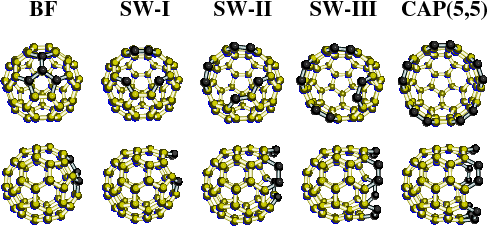
\includegraphics[width=12.5cm]{sample-fig1}}
		\caption[Enter the caption title here]{ Ball-and-stick models of meta-stable isomers in
			cage opening process from a C$_{60}$ buckminsterfullerene
			to a (5,5) capsule. We name them BF and CAP(5,5).
			Depending on the number of the Stone-Wales (SW) transformation,
			we call the intermediate isomers with SW-I, SW-II, and SW-III.
			Highlighted atoms are undercoordinated except BF.
		} \label{mag-fig1}
	\end{figure}

	\section{Application}

	The achievable rates can be calculated by finding the statistics of the five signals transmitted that maximize the mutual information between $s_{t,XY}$ and $y_{t,XY}$ for $(X,Y)=(T,C), (C,N)$, and $(N,C)$ when $t=1$, and $(X,Y)=(C,R), (C,N)$, and $(N,C)$ when $t=2$ \cite{SOCA2,EF2}...


	\chapter{Concluding Remark}

	We have proposed a novel FD MIMO-CCRN framework providing a reasonable performance improvement compared with the conventional MIMO-CCRN framework...
	%%
	%% 참고문헌 시작
	%% bibliography
	%% It can be changed but should include sufficient information.
%	\begin{thebibliography}{00}
%
%		\bibitem{FD1} 박상우, \underline{동시 송수신 안테나를 두 개 쓰는 협력 인지 무선통신망에 알맞은 전 이중 통신}, 한국과학기술원 석사 학위 논문, 2016.
%
%		\bibitem{RVP1} 송익호, 박철훈, 김광순, 박소령, \underline{확률변수와 확률과정}, 자유아카데미, 2014.
%
%		\bibitem{ML1} 송익호, 안태훈, 민황기, \underline{인지 무선에서의 광대역 주파수 검출 방법 및 장치}, 특허등록번호 10-1494966, 2015년 2월 12일.
%
%		\bibitem{SOCA1} 호우위시, 이원주, 이승원, 안태훈, 이선영, 민황기, 송익호, “선형 판별 분석에서 부류안 분산 행렬의 영 공간 재공식화,” \underline{한국통신학회 2012년도 추계종합학술발표회}, 대한민국 고려대학교, 242-243쪽, 2012년 11월.
%
%		\bibitem{EF1} 민황기, 안태훈, 이승원, 이성로, 송익호, “비간섭 전력 부하 감시용 고차 적률 특징을 갖는 전력 신호 인식,” \underline{한국통신학회논문지}, 제39C권, 제7호, 608-614쪽, 2014년 7월.
%
%
%
%		\bibitem{FD2} S. Park, \textit{Full-Duplex Communication for Cooperative Cognitive Radio Networks with Two Simultaneous Transmit and Receive Antennas}, Master Thesis, Korea Adv. Inst. Science, Techn., Daejeon, Republic of Korea, 2016.
%
%		\bibitem{RVP2}  I. Song, J. Bae, and S. Y. Kim, \textit{Advanced Theory of Signal Detection: Weak Signal Detection in Generalized Observations}, Springer-Verlag, 2002.
%
%		\bibitem{ML2} I. Song, T. An, and J. Oh, \textit{Near ML decoding method based on metric-first search and branch length threshold,} registration no. US 8018828 B2, Sep. 13, 2011, USA.
%
%		\bibitem{SOCA2} H.-K. Min, T. An, S. Lee, and I. Song, “Non-intrusive appliance load monitoring with feature extraction from higher order moments,” in \textit{Proc. 6th IEEE Int. Conf. Service Oriented Computing, Appl.,} Kauai, HI, USA, pp. 348-350, Dec. 2013.
%
%		\bibitem{EF2} I. Song and S. Lee, “Explicit formulae for product moments of multivariate Gaussian random variables,” \textit{Statistics, Probability Lett.,} vol. 100, pp. 27-34, May 2015.
%
%
%	\end{thebibliography}
%
%

	%%
	%% 감사의 글 시작
	%% Acknowledgement
	%%
	% @command acknowledgement 감사의글
	% @options [1 | 2 | 3 |4 ]
	% - 1 : 본문과 감사의 글이 둘 다 한글일 때  | 2 : 본문은 한글인데 감사의 글이 영어일 때 | 3 :  본문과 감사의 글이 둘 다 영어일 때  | 4 : 본문은 영어인데 감사의 글이 % 한글일 때
	%% It is optional.

	\acknowledgment[4]
	언제나 저를 바른 길로 이끌어 주시는 송익호 교수님께 큰 고마움을 느낍니다.
	끝으로 오늘의 제가 있을 수 있도록 사랑으로 키워 주신 가족들에게 감사드립니다.
	저의 이 작은 결실이 그분들께 조금이나마 보답이 되기를 바랍니다.

	%%
	%% 약력 시작
	%% Curriculum Vitae
	%%
	% @command curriculumvitae 이력서
	% @options [1 | 2 | 3 |4 ]
	% - 1 : 본문과 약력이 둘 다 한글일 때  | 2 : 본문은 한글인데 약력이 영어일 때 | 3 :  본문과 약력이 둘 다 영어일 때  | 4 : 본문은 영어인데 약력이 한글일 때
	%% It is optional and you can change form of this in the class file if you want.
	\curriculumvitae[4]

	% @environment personaldata 개인정보
	% @command     name         이름
	%              dateofbirth  생년월일
	%              birthplace   출생지
	%              domicile     본적지
	%              address      주소지
	%              email        E-mail 주소
	% - 위 6개의 기본 필드 중에 이력서에 적고 싶은 정보를 입력
	% input data only you want
	\begin{personaldata}
		\name       {힌릭스 예폐}
		\dateofbirth{1991}{07}{22}
		\birthplace {Aarhus}
		\address    {}
	\end{personaldata}

	% @environment education 학력
	% @options [default: (none)] - 수학기간을 입력
	\begin{education}
		\item[2008. 3.\ --\ 2010. 2.] 고등학교 (2년 수료)
		\item[2010. 2.\ --\ 2014. 2.] 한국과학기술원 물리학과 (학사)
		\item[2014. 3.\ --\ 2016. 2.] 한국과학기술원 전기및전자공학부 (석사)
	\end{education}

	% @environment career 경력
	% @options [default: (none)] - 해당기간을 입력
	\begin{career}
		\item[2015. 3.\ --\ 2016. 2.] 한국과학기술원 전기및전자공학부 조교
	\end{career}

	% @environment activity 학회활동
	% @options [default: (none)] - 활동내용을 입력
	%%    \begin{activity}
		%%        \item J. Choi, \textbf{Yong-Hyun Kim}, K.J. Chang, and D. Tomanek,
		%%             \textit{Occurrence of itinerant ferromagnetism in C/BN superlattice
			%%             nanotubes}, 5th Asian Workshop on First-Principles Electronic
		%%             Structure Calculations, Seoul (Korea), October., 2002.
		%%    \end{activity}

	% @environment publication 연구업적
	% @options [default: (none)] - 출판내용을 입력
	\begin{publication}
		%\item \textbf{Yong-Hyun Kim}, J. Choi, K.J. Chang, and D. Tomanek,
		%     \textit{Magnetic instability in partly opened C$_{60}$ isomers},
		%     in preparation.
		\item H.-K. Min, Y. Hou, {\bf S. Park}, and I. Song,
		``A computationally efficient scheme for feature extraction with kernel discriminant analysis,"
		\textit{Patt. Recogn.}, vol.~50, no.~2, pp.~45-55, Feb. 2016 (to be published).
	\end{publication}

	\label{paperlastpagelabel}     % <-- 추가 부분: 마지막 페이지 위치 지정
	%% 본문 끝
\end{document}
